\section{Introduction} \label{ICRA:sec:intro}

 Learning dynamics models for manipulation is an increasingly popular paradigm, in part because learned models can be repeatedly improved using autonomously collected real-world data. However, fine-tuning an initial dynamics model on new data can perform poorly when the data contains complex dynamics on which the dynamics model was not initially trained. For example, suppose we want to manipulate a rope amongst clutter, and we have a dynamics model trained on free-space motions in simulation. Free-space transitions in the real world are fairly similar to the free-space in simulation, but transitions where the rope deforms on objects in the scene are very different from anything seen in simulation. We call these transitions \emph{distracting}, because they are hard to learn from a few examples, and because they make it harder to adapt accurately to the free space dynamics. More generally, transitions from regions of dissimilar dynamics can inhibit effective transfer to regions of similar dynamics. This problem is similar to ``cleaning'' data in machine learning \cite{mislabeled99,filtering21,anomoly22}. For dynamics learning, defining what ``clean'' means can be difficult, and has not been studied extensively. Instead, the dominant paradigm is simply to train on all the collected data.

However, training on all the data can fail because real world datasets for learning dynamics are often too small to learn generalized models over the entire state-action space. In our experiments, we show that simply fine-tuning on all the data can yield a model that is not accurate enough for planning. If the task can be completed while remaining in regions where dynamics are similar, then it can be worth trading accuracy in dissimilar regions for accuracy in similar regions.
Our key insight is that, when we are adapting from an initial model, we can leverage the initial model to achieve significantly lower prediction error by focusing on transitions where the source and target dynamics are the most similar. The idea that transfer is easier when the source and target data are similar is well-supported in the transfer learning literature ~\cite{sorocky2020experience,bocsi2013alignment}. Concurrent work in offline reinforcement learning has also explored how staying closed to similar data leads to better policies \cite{vuong2022dasco}.

\begin{figure}
    \centering
    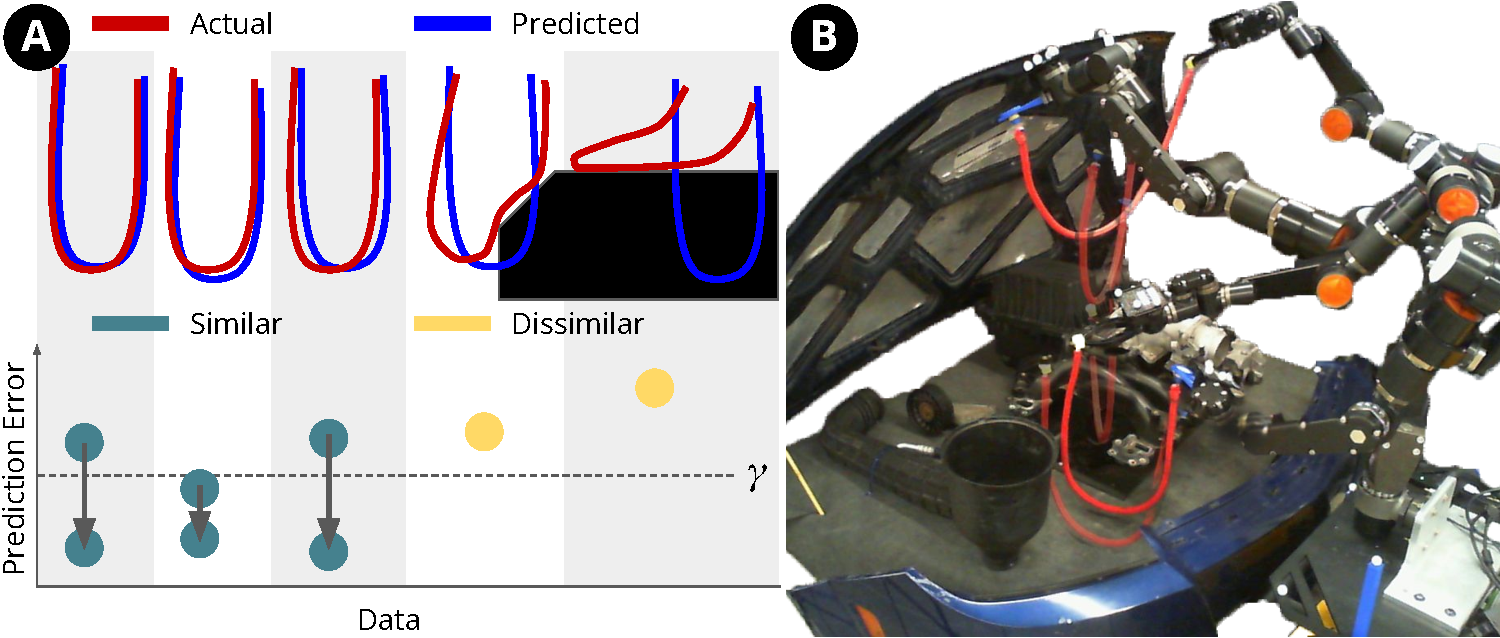
\includegraphics[width=1\linewidth]{Chap4/images/title_figure.pdf}
    \caption{
    (A) An illustration of how our adaptation method focuses on regions where the source and target dynamics are similar. When focusing adaption on free-space dynamics, the prediction errors decrease for other free-space data (similar), do not decrease for collision dynamics (dissimilar).
    (B) A mock-up of a car engine bay. The robot must move the rope and place it under the engine without snagging it to set up for lifting the engine. We use our proposed adaptation method to improve success rate during online learning for this task.}
    \label{ICRA:fig:real_robot_setup}
\end{figure}

To implement this strategy, we propose an adaptation method which minimizes prediction error in regions where the source and target dynamics are similar. The proposed method minimizes prediction error in these regions by fine-tuning on an initially small set of data from these regions, and growing that subset over the course of training. This is done with a loss function inspired by curriculum-learning that weighs transitions according to their prediction error, assigning higher weight to low-error transitions. Under the assumption that there are paths to the goal where the source and target dynamics are similar, this adaptation method can be used to achieve high task success in the target environment.

The first contribution of this chapter is a method for adapting dynamics models to datasets which contain distracting transitions. We demonstrate the proposed method is successful in filtering out distracting data and that the resulting trained model is more accurate in the regions of state-action space where the source and target dynamics are similar. The second contribution is a data-efficient online-learning method that pairs our adaptation method with prior work on planning with unreliable dynamics models \cite{UnreliableMitrano2021,MDEs22}. We call our combined method for online learning \FOCUS{}. \FOCUS{} achieves higher success rates in the low-data regime because the adapted dynamics are more accurate, which leads to finding more reliable plans.